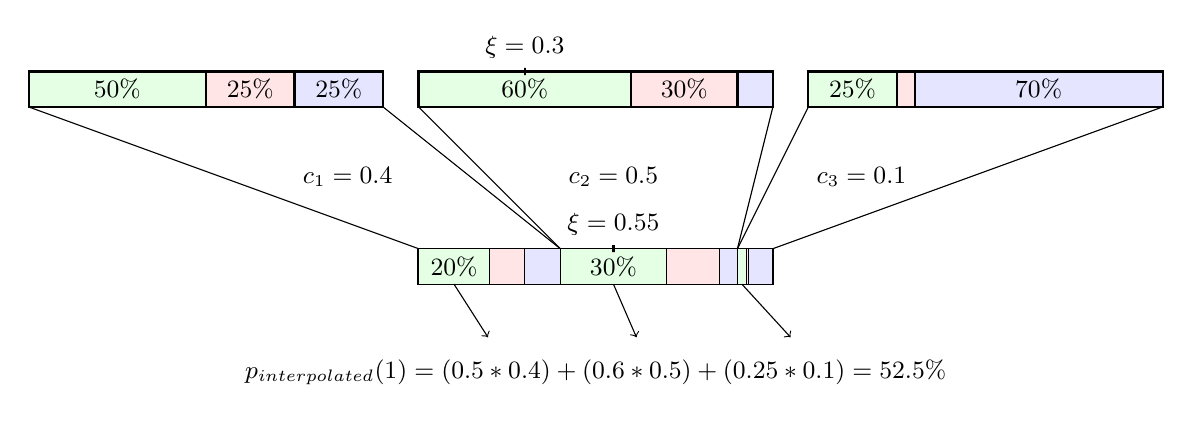
\begin{tikzpicture}[scale=4.5, cdf/.style ={thick}]
    \small
    %zoom lines
    \draw (-1.1,0) -- (0,-0.4);
    \draw (-0.1,0) -- (0.4,-0.4);
    \draw (0,0) -- (0.4,-0.4);
    \draw (1,0) -- (0.9,-0.4);
    \draw (1.1,0) -- (0.9,-0.4);
    \draw (2.1,0) -- (1,-0.4);
    
    \draw[cdf] (-1.1,0) rectangle (-0.1,0.1);
    \draw[cdf] (0,0) rectangle (1,0.1);
    \draw[cdf] (1.1,0) rectangle (2.1,0.1);
    \draw[cdf] (0,-0.5) rectangle (0.4,-0.4);
    \draw[cdf] (0.4,-0.5) rectangle (0.9,-0.4);
    \draw[cdf] (0.9,-0.5) rectangle (1,-0.4);
    
    %cdfs, lines and filling
    \draw[thick, fill=green!10] (-1.1,0) rectangle (-0.6, 0.1) node[pos=.5] {50\%};
    \draw[thick, fill=red!10] (-0.6, 0) rectangle (-0.35, 0.1) node[pos=.5] {25\%};
    \draw[thick, fill=blue!10] (-0.35, 0) rectangle (-0.1, 0.1) node[pos=.5] {25\%};
    
    \draw[thick, fill=green!10] (0,0) rectangle (0.6, 0.1) node[pos=.5] {60\%};
    \draw[thick, fill=red!10] (0.6, 0) rectangle (0.9, 0.1) node[pos=.5] {30\%};
    \draw[thick, fill=blue!10] (0.9, 0) rectangle (1, 0.1);
    
    \draw[thick, fill=green!10] (1.1,0) rectangle (1.35, 0.1) node[pos=.5] {25\%};
    \draw[thick, fill=red!10] (1.35, 0) rectangle (1.4, 0.1);
    \draw[thick, fill=blue!10] (1.4, 0) rectangle (2.1, 0.1) node[pos=.5] {70\%};
    
    \draw[fill=green!10] (0,-0.5) rectangle (0.2,-0.4) node[pos=.5] {20\%};
    \draw[fill=red!10] (0.2,-0.5) rectangle (0.3,-0.4);
    \draw[fill=blue!10] (0.3,-0.5) rectangle (0.4,-0.4);

    \draw[fill=green!10] (0.4,-0.5) rectangle (0.7,-0.4) node[pos=.5] {30\%};
    \draw[fill=red!10] (0.7,-0.5) rectangle (0.85,-0.4);
    \draw[fill=blue!10] (0.85,-0.5) rectangle (0.9,-0.4);
    
    \draw[fill=green!10] (0.9,-0.5) rectangle (0.925,-0.4);
    \draw[fill=red!10] (0.925,-0.5) rectangle (0.93,-0.4);
    \draw[fill=blue!10] (0.93,-0.5) rectangle (1,-0.4);
    
    \draw[thick] (0.55,-0.39) node[above] {$\xi = 0.55$} rectangle (0.55,-0.41);
    
    \draw[thick] (0.3, 0.11) node[above] {$\xi = 0.3$} rectangle (0.3,0.09);
    
    \node at (0.5, -0.75) {$p_{\text{interpolated}}(1) = \overbracket{(0.5 * 0.4)} + \overbracket{(0.6 * 0.5)} + \overbracket{(0.25 * 0.1)} = 52.5\%$};
    
    \draw[->] (0.1,-0.5) -- (0.196,-0.65);
    \draw[->] (0.55,-0.5) -- (0.615,-0.65);
    \draw[->] (0.9125,-0.5) -- (1.05,-0.65);
    
    % pi range indicators
    \path (-0.2, -0.25) node[above] {$c_1 = 0.4$};
    \path (0.55, -0.25) node[above] {$c_2 = 0.5$};
    \path (1.25, -0.25) node[above] {$c_3 = 0.1$};
    
\end{tikzpicture}